\documentclass[border=10pt]{standalone}

\usepackage{tikz}
\usepackage{tikzsymbols}
\usetikzlibrary{calc,patterns,shapes.geometric}

\def\centerarc[#1](#2)(#3:#4:#5){\draw[#1] ($(#2)+({#5*cos(#3)},{#5*sin(#3)})$) arc (#3:#4:#5);}

\begin{document}
	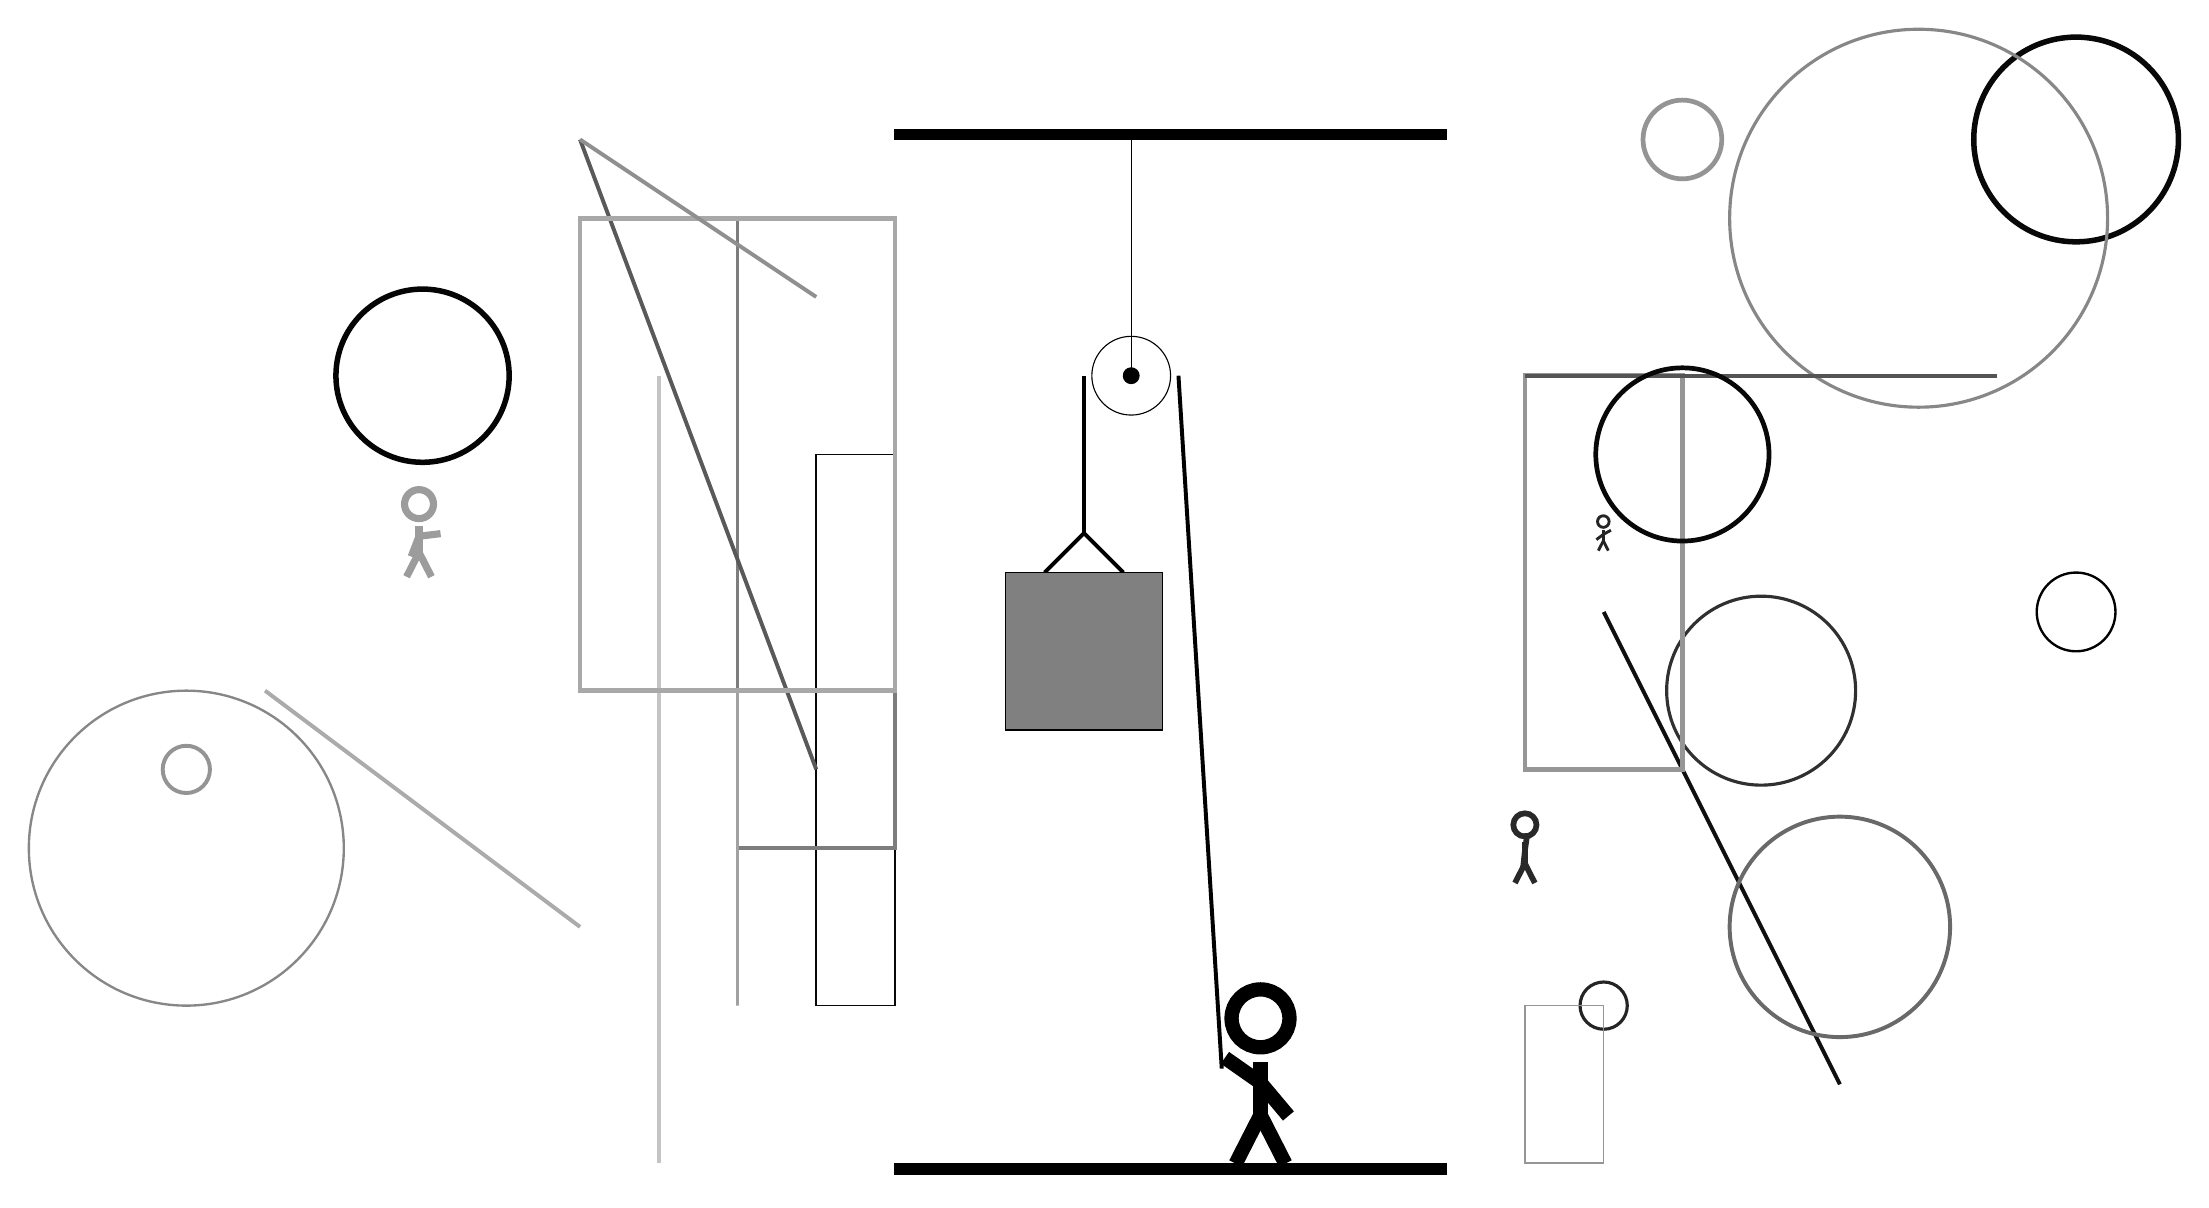
\begin{tikzpicture}
		%%%%% START %%%%%
		
		\draw[fill=black] (-2, 10) rectangle (5, 10.125);
		
		\draw (1, 7) circle (0.5);
		\draw[fill=black] (1, 7) circle (0.1);
		\draw (1, 10) -- (1, 7);
		
		\draw[line width=0.5mm] (-0.1, 4.5) -- (0.4, 5.0) -- (0.9, 4.5);
		\draw[fill=black!50] (-0.6, 4.5) rectangle (1.4, 2.5);
		
		\draw[line width=0.2mm, color=black!97] (-3, 6) rectangle (-2, -1);
		
		\draw [line width=0.4mm, color=black!81](9, 3) circle (1.2);
		\draw [line width=0.7mm, color=black!97](13, 10) circle (1.3);
		\draw[line width=0.5mm, color=black!23](-5, -3) -- (-5, 7);
		\draw [line width=0.5mm, color=black!42](-11, 2) circle (0.3);
		
		\draw[line width=0.5mm, color=black!94](10, -2) -- (7, 4);
		\draw [line width=0.4mm, color=black!47](11, 9) circle (2.4);
		\draw [line width=0.5mm, color=black!59](10, 0) circle (1.4);
		\draw[line width=0.5mm, color=black!51] (-4, 9) rectangle (-2, 1);
		
		\draw[line width=0.5mm, color=black!33](-6, 0) -- (-10, 3);
		\draw[line width=0.6mm, color=black!41] (6, 2) rectangle (8, 7);
		\node[line width=0.6mm, color=black!39] at (-8, 5) {\Strichmaxerl[5][69][7]};
		\draw [line width=0.7mm, color=black!98](-8, 7) circle (1.1);
		
		\draw [line width=0.4mm, color=black!86](7, -1) circle (0.3);
		\draw[line width=0.5mm, color=black!67](6, 7) -- (12, 7);
		\draw[line width=0.5mm, color=black!65](-3, 2) -- (-6, 10);
		
		\draw [line width=0.6mm, color=black!42](8, 10) circle (0.5);
		\node[line width=0.3mm, color=black!84] at (6, 1) {\Strichmaxerl[4][84][82]};
		\draw[line width=0.3mm, color=black!37] (-4, 3) rectangle (-4, -1);
		\draw [line width=0.6mm, color=black!97](8, 6) circle (1.1);
		\draw [line width=0.3mm, color=black!100](13, 4) circle (0.5);
		
		\draw[line width=0.6mm, color=black!34] (-2, 9) rectangle (-6, 3);
		\node[line width=0.2mm, color=black!86] at (7, 5) {\Strichmaxerl[2][37][29]};
		\draw [line width=0.3mm, color=black!47](-11, 1) circle (2.0);
		\draw[line width=0.5mm, color=black!44](-6, 10) -- (-3, 8);
		\draw[line width=0.2mm, color=black!41] (6, -3) rectangle (7, -1);
		
		\draw[line width=0.5mm] (0.4, 7) -- (0.4, 5.0);
		\centerarc[line width=0.5mm](1, 7)(0:180:0.6);
		\draw[line width=0.5mm](1.6, 7) -- (2.15, -1.8);
		
		\node at (2.6, -1.9) {\Strichmaxerl[10][-35][-50]};
		
		\draw[fill=black] (-2, -3) rectangle (5, -3.15);
		
		%%%%% END %%%%%
	\end{tikzpicture}
\end{document}